% \begin{multicols}{2}
\chapter{Evaluation}
In this part, using the trained LSTM RNN model in last section to make 
predictions on pandemic and post-pandemic date sets. 
Evaluate the results of the predictions and 
assess the impact of the pandemic on Dublin city-bike usage.
\section{Predictions}
Using the trained model to make predictions on pandemic period and 
post pandemic bike-usage data. 
Comparing the predictions with the collected data to assess the impact of 
pandemic.
Without considering the usage specifically for each station, 
generally predict the full dataset is the simple way to assess the differences.
The \ref{FIGURES: Predictions Samples of Pandemic Period}
shows a brief view of predictions and sample values.
Although there are differences can be determine from the figures 
(post-pandemic period \ref{FIGURES: Predictions Samples of POST Pandemic Period}
and pandemic period \ref{FIGURES: Predictions Samples of Pandemic Period}), 
the qualitative analysis should be applied.

\paragraph{Qualitative Analysis}
In order to determine the differences between theoretical prediction and the 
real values, there are many methods to do so. 
\begin{figure}[H]
    \centering
    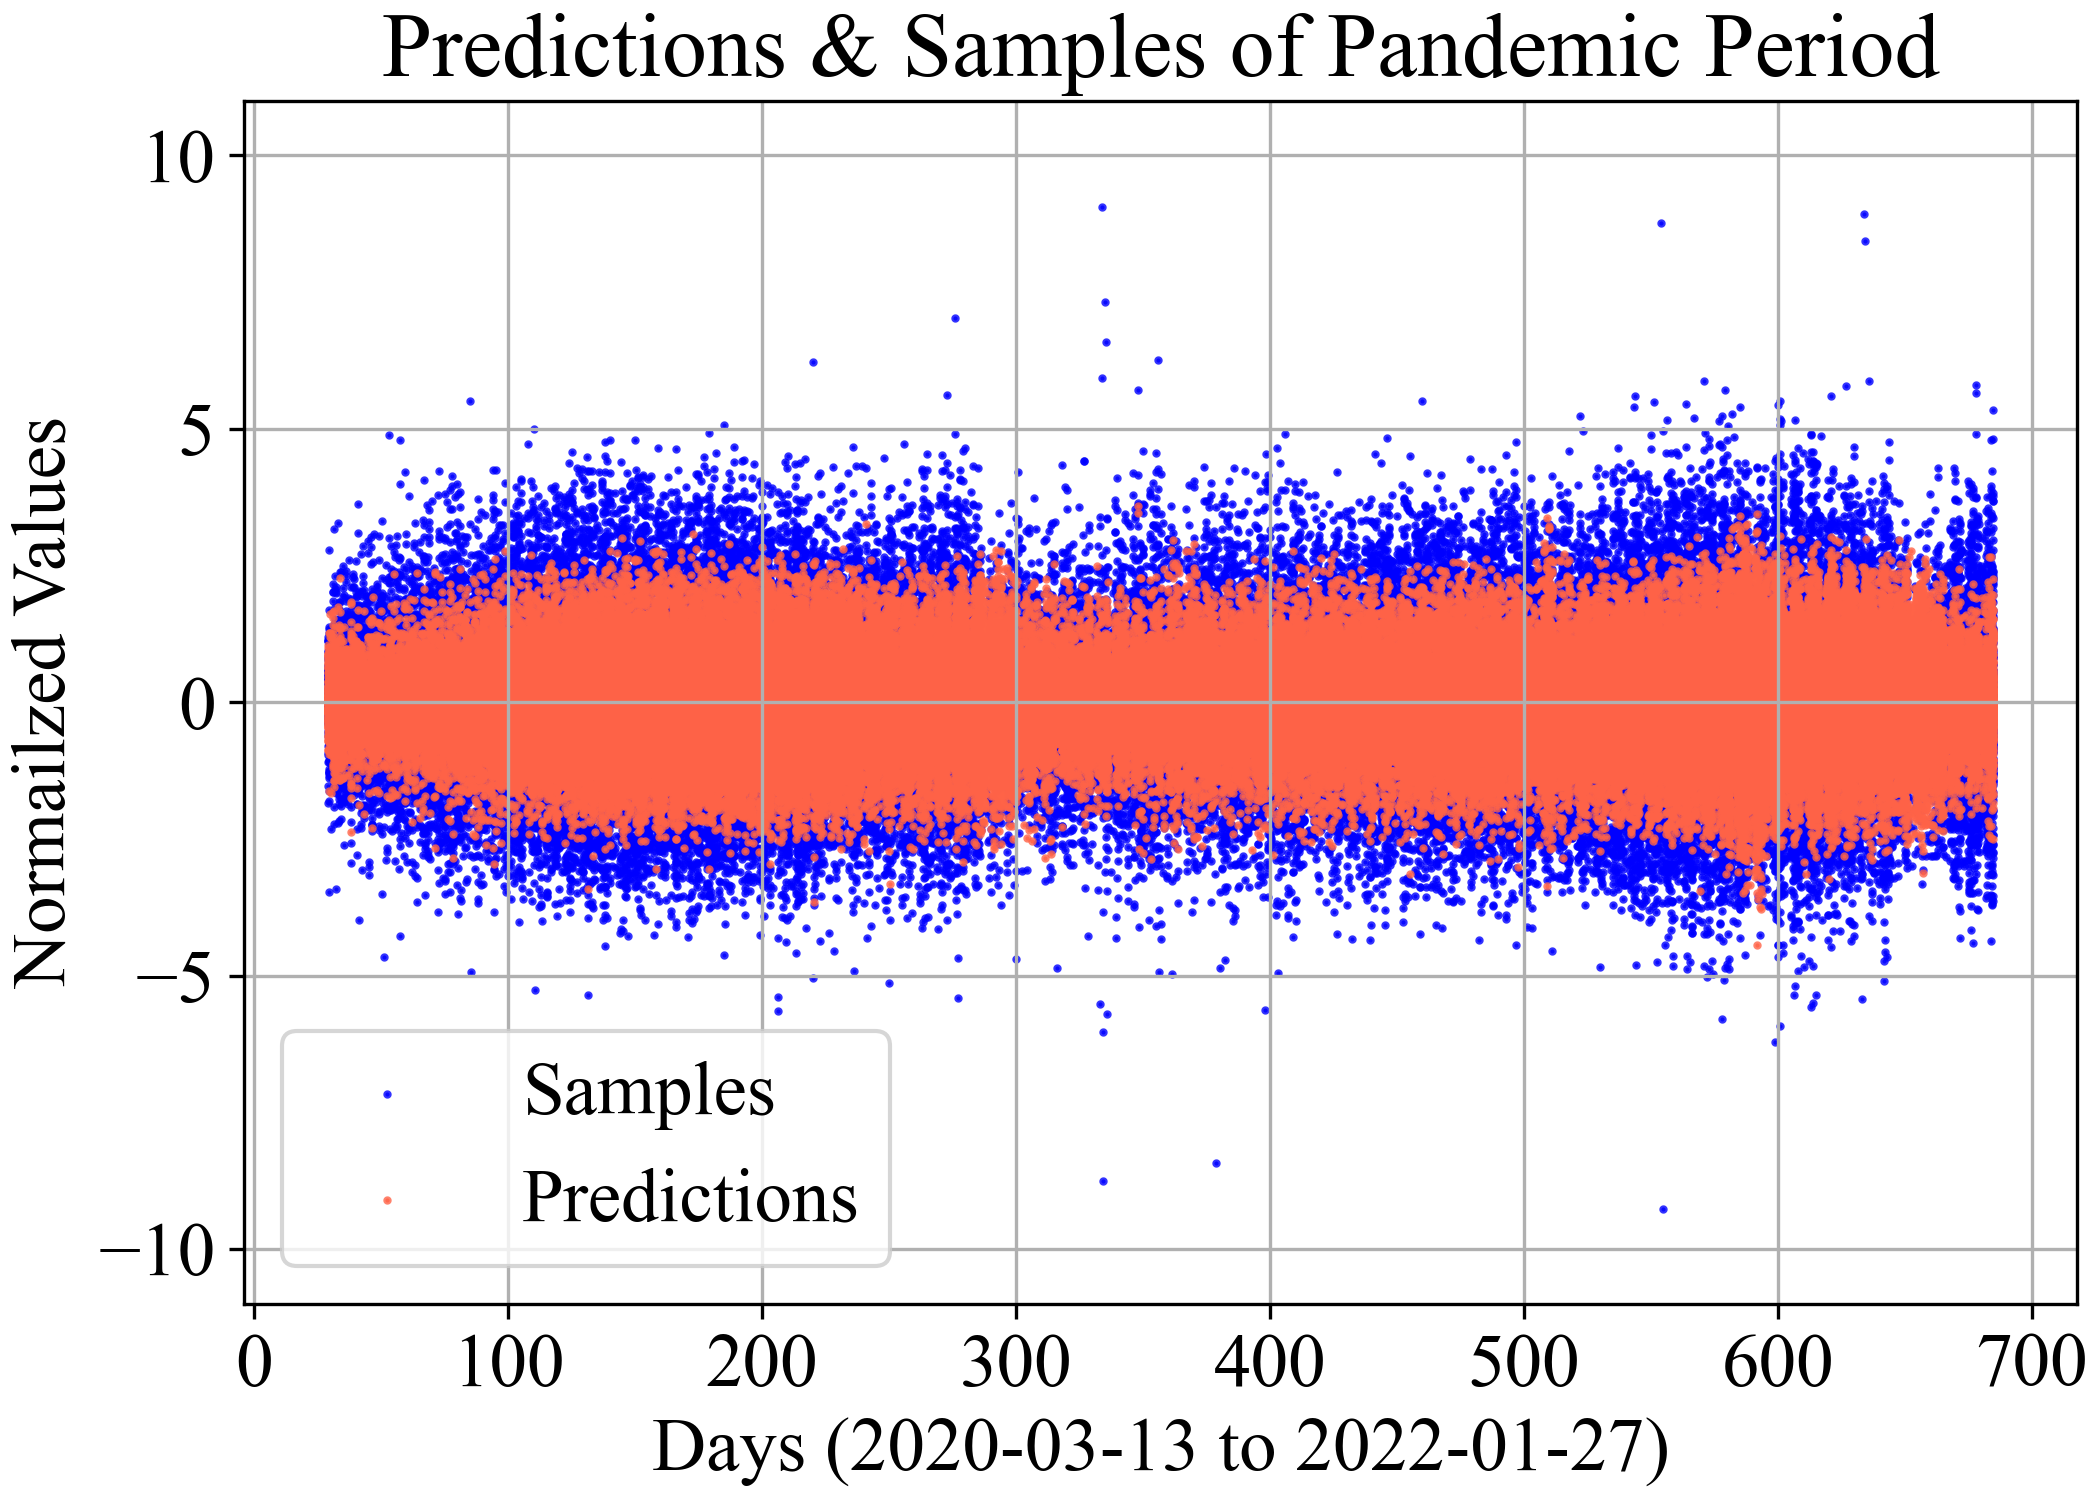
\includegraphics[width=0.45\textwidth]{chap/fig5.png}
    \caption{
        \footnotesize 
            Predictions \& Samples of Pandemic Period
        } % 表格标题
    \label{FIGURES: Predictions Samples of Pandemic Period}
\end{figure}
But for simply purpose rather than the most precisely purpose, 
using the 'Bootstrap' to analysis the results since it is an 
efficient method to evaluate the performance and the reliance of model.

In this case specifically, randomly select a part of ($20\%$) the given dataset,
and evaluate the performance of the model on this fraction of sample. 
Totally, this process is looped $1000$ iterations. 
In more complex cases, the size of selected data samples and the number of iterations
are also required to determine by fine-tuning methods, since they are hyperparameter
as well. 
The 
\begin{figure}[H]
    \centering
    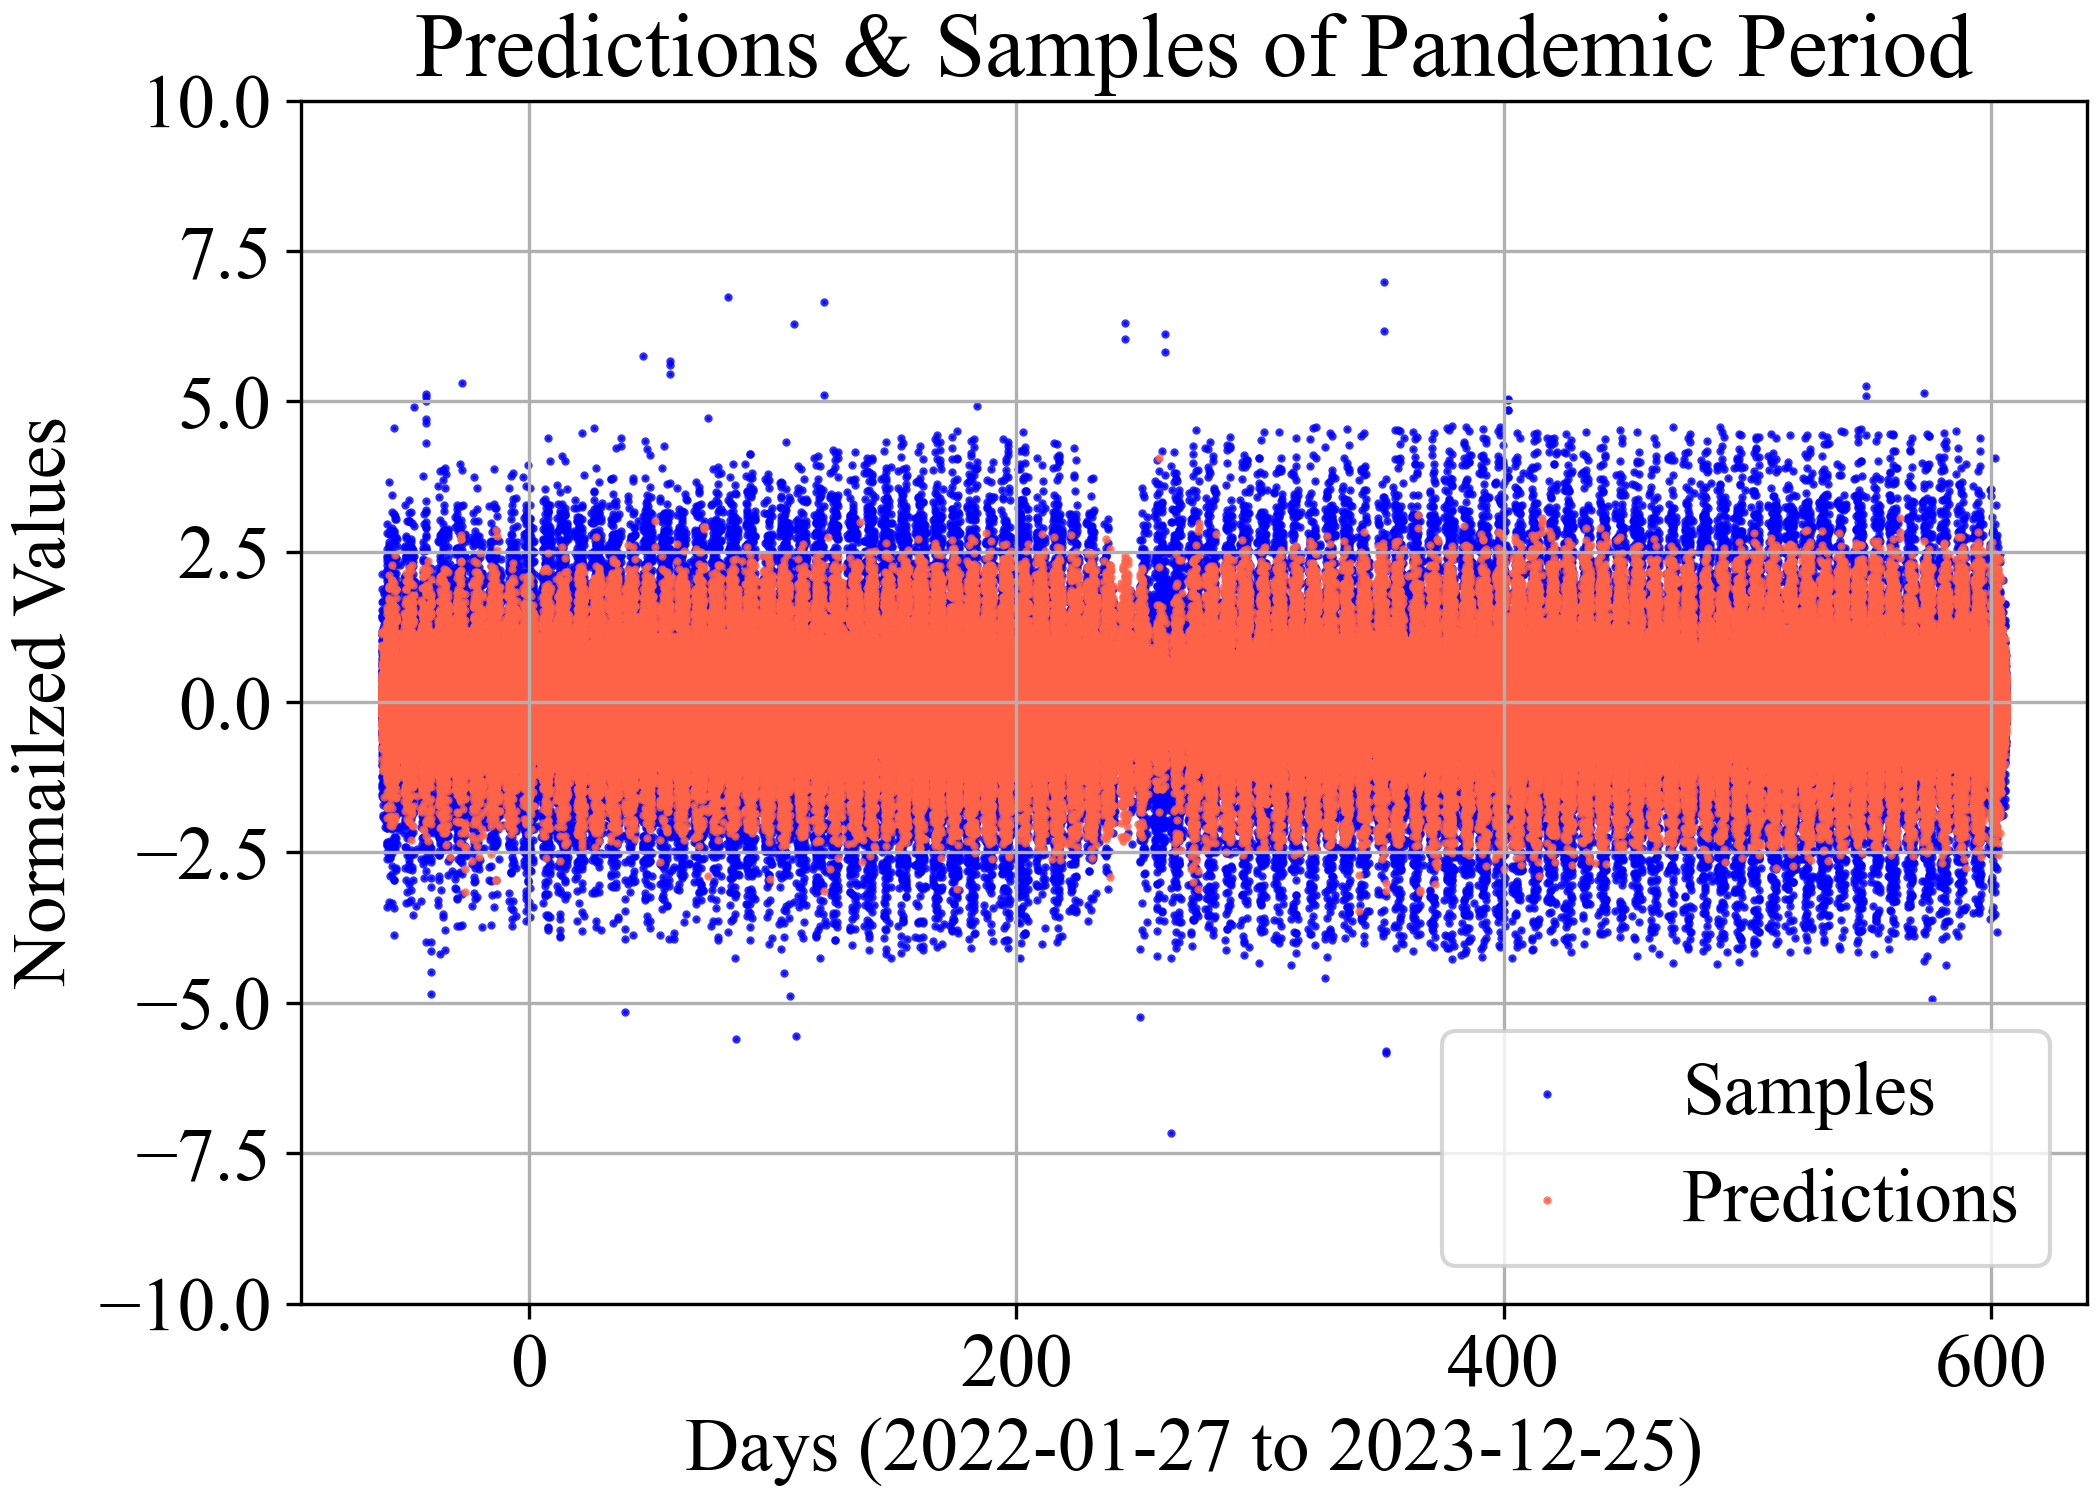
\includegraphics[width=0.45\textwidth]{chap/fig6.png}
    \caption{
        \footnotesize 
            Predictions \& Samples of Post-Pandemic Period
        } % 表格标题
    \label{FIGURES: Predictions Samples of POST Pandemic Period}
\end{figure}
The results of Bootstrap are shown in the table below \ref{TABLE: BOOTSTRAP DUR POST PRE } 
\begin{table}[H]
    \footnotesize
    \centering
        \caption{
            \footnotesize
            Mean \& standard deviation of Bootstrap results
        } % 表格标题
    \begin{tabular}{cccc} % 5列,全部居中对齐
        \toprule % 顶线
        periods & pre-pandemic & pandemic & post-pandemic \\ % 表头
        \midrule % 中线
        mean & 0.42277 & 0.8149587 & 0.478253  \\ % 第一行数据
        std & 0.00581216 & 0.0106626 & 0.005191669 \\ % 第一行数据
        \bottomrule % 底线
    \end{tabular}
    \label{TABLE: BOOTSTRAP DUR POST PRE
    } % 用于引用表格的标签
\end{table}
\paragraph{Discussion of pandemic period}
In \ref{TABLE: BOOTSTRAP DUR POST PRE }, it is clear to determine 
that the mean value of scores of Bootstrap (mse) in pandemic period
are much more higher than pre and post pandemic period, the 
standard deviation as well. 
It means that the impact of the pandemic to the bike-usage are 
significantly large compare to before and after it happened.
Also, it shows that the bike-usage in pandemic period 
are more unstable.

\paragraph{Discussion of post-pandemic period}
In \ref{TABLE: BOOTSTRAP DUR POST PRE }, comparing to the pre-pandemic and 
pandemic period, the bike-usage is slightly larger than pre-pandemic but 
much more smaller than pandemic period. 
It means that the bike-usage was sufficiently recovered after city lock-down ended.
And the bike-usage approximately recovered to the level as pre-pandemic period.
Besides that, the trend of bike-usage recovery is stable through 
observing the deviation which is approximately same but still smaller than pre-pandemic 
period. 